%*******************************************************************************
%****************************** Second Chapter *********************************
%*******************************************************************************

\chapter{Implementations}

\ifpdf
    \graphicspath{{Chapter5/Figs/Raster/}{Chapter5/Figs/PDF/}{Chapter5/Figs/}}
\else
    \graphicspath{{Chapter5/Figs/Vector/}{Chapter5/Figs/}}
\fi

\section{Architecture}

\begin{figure}[h!] 
\centering    
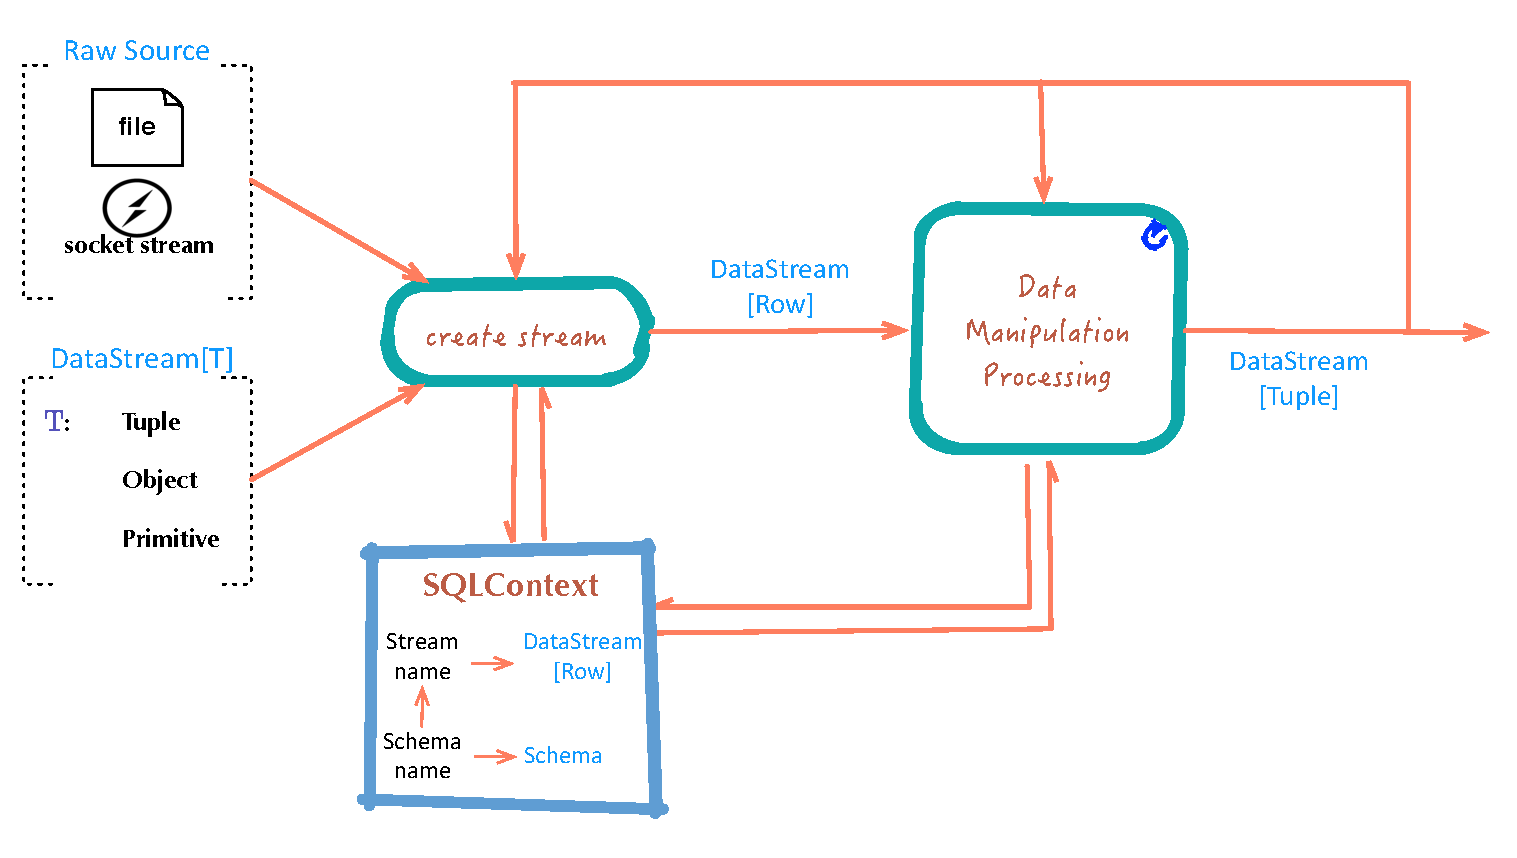
\includegraphics[width=1\textwidth]{Architecture}
\caption{Architecture}
\label{fig:Architecture}
\end{figure}


Figure~\ref{fig:Architecture} depicts the overall architecture of FlinkCQL query processing layer. It accepts data streams, query string and SQLContext as inputs and return one or more output data streams.
\subsection{Input Sources}
The query processing layer can connect to and process data streams from different data sources like file sources, web sockets, message queues (Apache Kafka, RabbitMQ, Twitter Streaming API …), and also from any user defined data sources. We classify the sources into 2 categories: \textit{Raw source} and predefined \textit{DataStream[T]} with \textit{T} is the type of elements.

\subsubsection*{Raw Source}


\textbf{Text file stream}: the source stream contains the lines of the files created (or modified) in a given directory. The system continuously monitors the given path, and processes any new files or modifications. The file will be read with the system’s default character set. FlinkCQL expresses the text file stream source via ``SOURCE FILE ( \textit{filePath, delimiter})'', the default delimiter is a comma. The delimiter is used to tokenize string and convert its result into tuples according to a schema


\textbf{Socket text stream}: the source stream contains the strings received from the given socket. Strings are decoded by the system’s default character set. Socket text stream is specified in FlinkCQL as ``SOURCE SOCKET ( \textit{filePath, delimiter})''
The user can optionally set a delimiter for the same purpose as in Text file stream.


\textbf{Message queue connectors:} There are pre-implemented connectors for a number of popular message queue services. Connectors provide an interface for accessing data from various third party sources (message queues). Currently three connectors are natively supported, namely Apache Kafka, RabbitMQ and the Twitter Streaming API. In the recent prototype of FlinkCQL, we have not designed any syntax for those connectors due to lacking of testing facilities. However, in the next prototype, we could extend its syntax at ease.

\subsection*{DataStream[T]}
The \textit{DataStream[T]} is the basic data abstraction provided by Flink Streaming. It represents a continuous, parallel, immutable stream of data of a certain type \textit{T}. Type \textit{T} could be :
\begin{itemize}
\item Primitive data type: integer, double, ...
\item Tuple type: which is a composite of multiple primitive data types such as \textit{(integer, string, integer)}
\item Class object: such as \textit{CarEvent(id: Int, speed: Int)}
\end{itemize} 

\subsection{SQL Context} 

At the beginning, we encounter a problem of diverse data types of stream elements. A source stream can contains elements of string type (as in raw source), other primitive types, tuple or class instance. It is cumbersome and impractical to provide query processing for all kinds of source streams respectively. Thus, when a data stream is entitled to a schema (via \textit{Create Stream} or \textit{Insert} statement), we first transform the origin source stream to a Data Stream of a universal type \textit{Row} . \textit{Row} is simply a tuple containing \textit{an array of any data} including \textit{Null}. We do not specify the type of elements inside the Row. Those types will be derived from Schema.

Recall the example in ~\ref{query:createStream} to create schema and stream of ``StockTick''.
\begin{lstlisting}
	CREATE SCHEMA StockTickSchema (symbol String, sourceTimestamp Long, price Double, quantity Int, exchange String)
\end{lstlisting}

\begin{lstlisting} 
	CREATE STREAM StockTick StockTickSchema 
	SOURCE SOCKET ("98.138.253.109", 2000)
\end{lstlisting}

``StockTick'' is the Stream used inside FlinkCQL query. It is entitled to ``StockTickSchema'' and mapped to a real \textit{DataStream[Row]} which is derived from the socket text stream. The correlation between Stream and Schema is expressed in Figure~\ref{fig:SQLContext}. Be aware that the concept of Stream in FlinkSQL and DataStream in Flink is not identical. In fact, a Stream in FlinkSQL is a name to represent a \textit{DataStream[T]} in Flink.

All Stream-Schema-DataStream relationships are stored in 3 dictionaries of \textit{SQLContext}~(Figure~\ref{fig:Architecture}). 
Stream and Schema are unique but many Stream can share a Schema. And a Stream is mapped to a DataStream[T]. When user send out some further queries, query processing framework will lookup \textit{SQLContext} to decide which Stream-Schema is specified to generate an precise snippet of code.

\begin{figure}[h!] 
\centering    
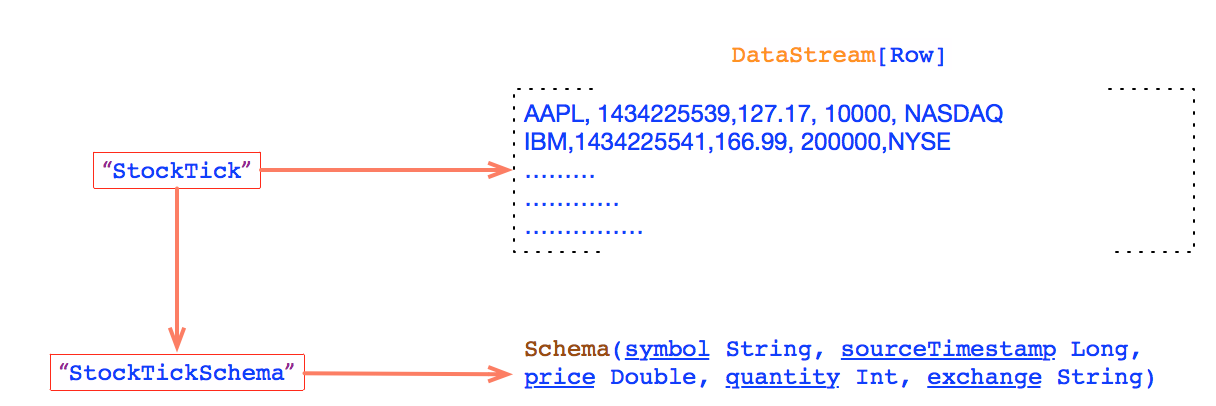
\includegraphics[width=0.8\textwidth]{SQLContext}
\caption{\textit{Stream}-\textit{Schema} mapping in \textit{SQLContext}}
\label{fig:SQLContext}
\end{figure}

\subsection{Data Manipulation Processing}
Data Manipulation Processing is used to process Data Manipulation Queries such as SELECT, MERGE, SPLIT, INSERT. These queries specify which operators to process on given Streams and its Fields. System will look up its SQLContext to retrieve the actual input DataStream[Row]. Operator and Schema are to decide how to transform input DataStreams to a new one. The output of processing is either one or more Streams which are updated into SQLContext or a DataStream of tuple. This DataStream of tuple can be consumed to create other Stream via \textit{CREATE STREAM} query. For examples, the output of \textit{SELECT} query is a DataStream of tuple but the outputs of \textit{SPLIT} query are more than one Stream~(along with its Schema and DataStream[Row]).

\section{FlinkCQL Query Interpreter}
\begin{figure}[h!] 
\centering    
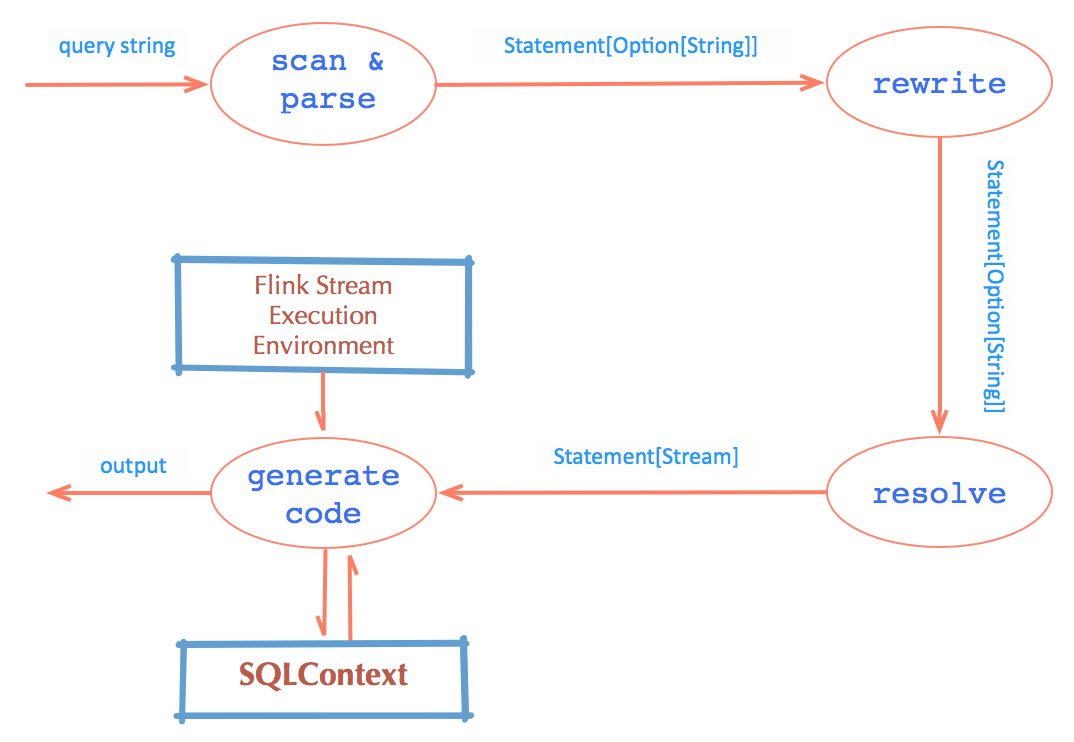
\includegraphics[width=0.7\textwidth]{QueryProcessing}
\caption{Query Processing}
\label{fig:QueryProcessing}
\end{figure}


//TODO: Tree-Based Interpreter~\citep{Parr:2009}
[Programming Language Pragmatics, Third Edition.pdf page 57


Flink Stream Processing is offering a rich set of API to deal with one or  multiple input DataStream[T]. Our goal is to build an extension which accepts FlinkCQL query strings as commands and translate the commands to  corresponding programs constructed with Flink's APIs. Thus we are simply required to build a interpreter instead of a compiler from a scratch. For the purpose, I have implemented a tree-based interpreter~\citep{Parr:2009} to process FlinkCQL query. The idea is that the query interpreter executes program by constructing an abstract syntax tree~(AST) from the input query string and walking through the tree to generate a executable Flink program. More specifically, AST is a form of intermediate representation of the hierarchical syntactical structure of the source program written in query.  
	

The interpretation proceed through a series of well-defined phrases (Figure~\ref{fig:QueryProcessing}). Each phrase transforms or extracts information of use from the output of previous phrase and return a result which is a input of next phrase. In first proof-of-concept prototype, we build a pipeline consisting of 4 steps:
\begin{itemize}
	\item \textbf{Scanning and parsing:} serve to recognize the structure of the program, without regard to its meaning. This steps produce an AST with its root is highest semantic level of query : \textit{Statement[Option[String]]}

	\item \textbf{Rewriting} is to modify a sub-tree of AST to a more compact, optimal AST without changing the semantic of program.
	
	\item \textbf{Resolving:} It is possible that two or more streams, which are specified in query,  shares the same Schema. Thus, there is a potential ambiguity between two fields which have a identical name but belong to different stream. This phrase is to figure out to which fields refers. It is clear that we cannot generate code from an ambiguous AST.
	
	\item \textbf{Code generation}: In addition to a compact and unambiguous AST, the interpreter also lookup Stream-Schema information from SQLContext to generate a Flink program based on pre-defined translation rules. Last but not at least, we need the Flink stream execution environment to execute our generated code.
	
I describe all phrases in following: 
	
\end{itemize}
\subsection{Scanning and Parsing}


 Heterogeneous AST

[Manning.DSLs.in.Action.pdf
Packrat parsing for left recursive DSL syntax

A DSL that needs a packrat parser


\begin{itemize}
	\item Step 1: Executing the grammar
	\item Step 2: Building the semantic model for the DSL
	\item Step 3: Designing the Order abstraction
	\item Step 4: Generating the AST using function application combinators
\end{itemize}




\begin{figure}[h!] 
\centering    
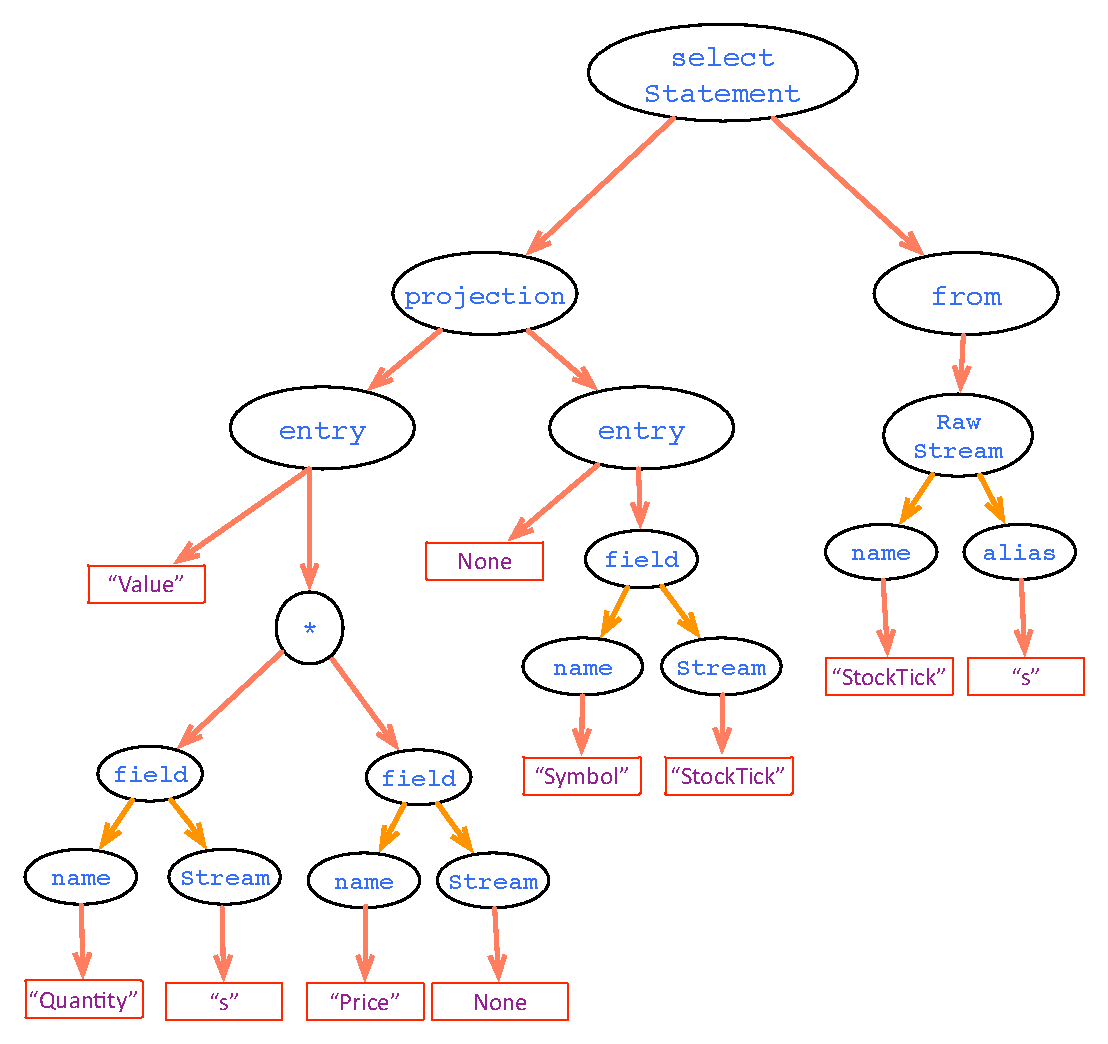
\includegraphics[width=0.7\textwidth]{Parse}
\caption{Parse}
\label{fig:Parse}
\end{figure}


\subsection{Query Rewriting}
Pattern Matching

We apply one rewriting rule for subquery:
\begin{lstlisting}
From (select Symbol,Price From StockTick [Size 3]) as s
=
From (select Symbol,Price From StockTick) [Size 3] as s
\end{lstlisting}

In the first query , its subquery will return a Windowed Stream which is not supported now. Therefore the query is invalid

In the second query, its subquery return a concrete DataStream which is acceptable.

However, the 2 queries are identical in term of semantics. Thus, we transform the first to the second.


\subsection{Resolving}
\begin{figure}[h!] 
\centering    
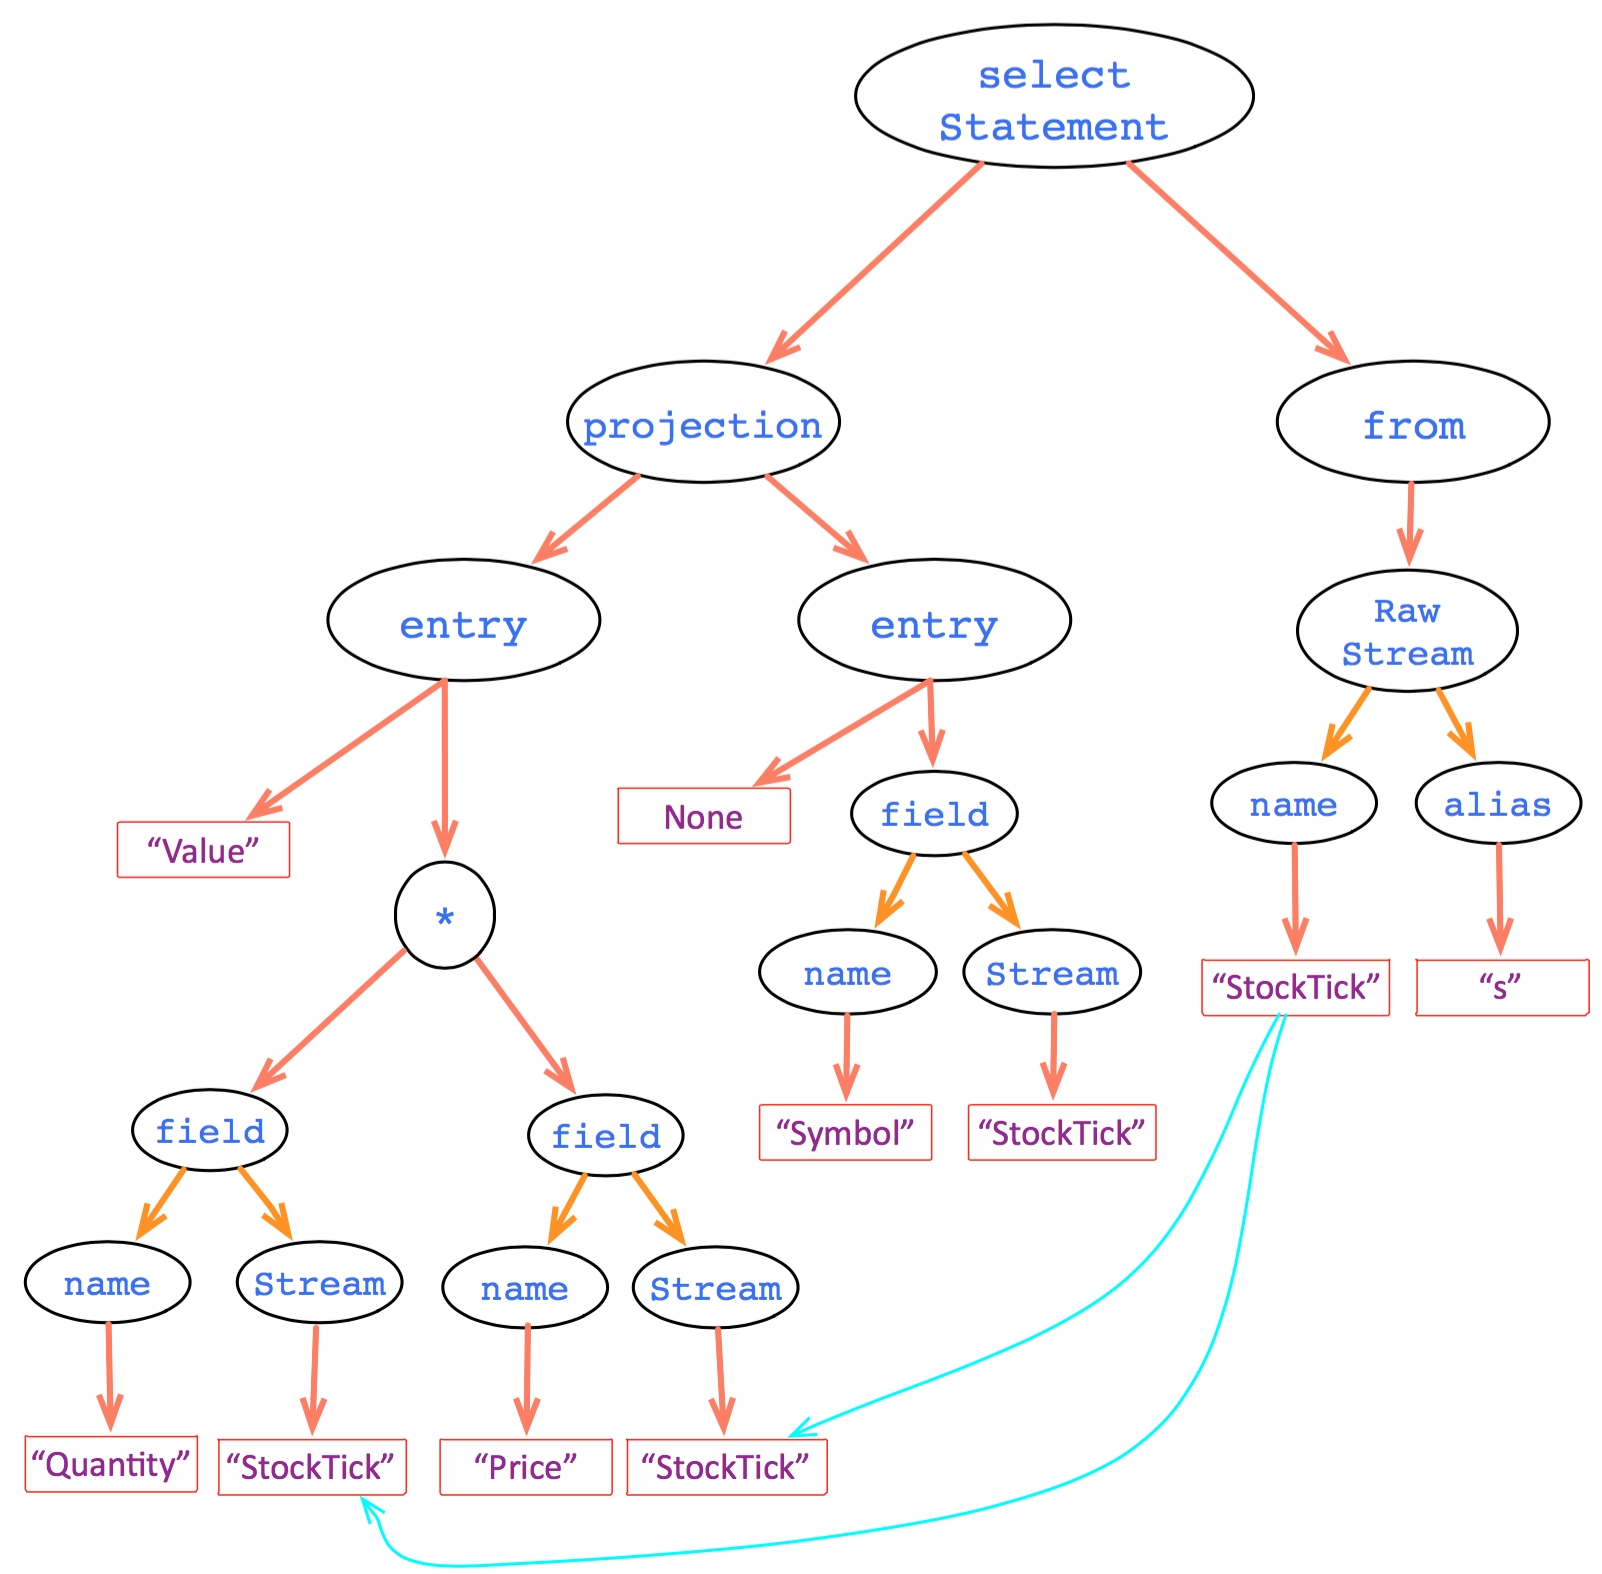
\includegraphics[width=0.7\textwidth]{Resolve}
\caption{Resolve}
\label{fig:Resolve}
\end{figure}

Pattern Matching
15 Tree pattern matcher


In the example, we are going to figure out  which streams that “StockTick.Symbol”, “s.Quantity”, “Price”  projections refer to. This step is important because perhaps many different streams have 2 fields which have an identical name. For example, 2 streams may own a field which is “Price”. 
This step helps to resolve which fields belongs to which streams so that we can generate the exact code for the query


\subsection{Code Generation}
Using Scala compile-time and run-time reflection to build a Scala Abstract Syntax Tree


Translation Rule


\section{Evaluations}

Compare to other systems


\section{Future Works}

Dynamic variable


http://www.sqlstream.com/blog/2015/03/5-reasons-why-spark-streamings-batch-processing-of-data-streams-is-not-stream-processing/



Data Input
http://flink.apache.org/news/2015/05/11/Juggling-with-Bits-and-Bytes.html


http://ci.apache.org/projects/flink/flink-docs-master/internals/fig/stack.svg

http://ci.apache.org/projects/flink/flink-docs-master/internals/general\_arch.html